\documentclass[11pt,aspectratio=1610,dvipsnames]{beamer}
\graphicspath{{figs/}}
\usetheme{default}
\usepackage{DasBeamerPaket}
\usepackage{animate}
\usepackage{lastpage}
\usepackage{tikz}
\setbeamercolor{section in toc}{fg=NavyBlue}
\setbeamercolor{frametitle}{fg=NavyBlue}
\captionsetup[figure]{labelfont=bf}
\captionsetup[table]{labelfont=bf}
\setbeamertemplate{caption}[numbered]
\newcommand{\btheta}{\boldsymbol{\theta}}
\begin{document}
\author{{\Large Dominic Schüchter}\\ \scriptsize \href{mail:dschuechter@uni-bonn.de}{\faEnvelope  \hspace*{0.1cm}dschuechter@uni-bonn.de} {\color{black}$|$} \href{https://github.com/dschuechter}{\faGithub  \hspace*{0.1cm}dschuechter}}
\title{Bayesian model selection}
\subtitle[Seminar physics760]{\textsc{Seminar physics760-Computational Physics}}
\logo{
\includegraphics[width=1cm]{UniBonnLogo}\vspace{235pt}\hspace{8pt}}

\date{\includegraphics[width=1.3cm]{institutelogo}\hspace{10px}
\includegraphics[width=1.3cm]{UniBonnLogo}}
\date{\includegraphics[width=8cm]{Titelbild.png}}
\definecolor{myWhite}{rgb}{1,1,1}

\setbeamertemplate{footline}[text line]{\parbox{0.3\linewidth}{\vspace*{-9pt}\textcolor{white} \insertsection  \hfill} \parbox{0.7\linewidth}{\vspace*{-8pt} \textcolor{white}{\hfill\hspace{-3cm}\insertshorttitle \phantom{ }-- \insertshortsubtitle}  \hfill \textcolor{myWhite}{\insertpagenumber/\pageref{LastPage}}}}

\addtobeamertemplate{footline}{ \makebox[0pt][l]{\hspace{-1cm}
		\raisebox{0cm}[0pt][0pt]{\colorbox{gray!15!black}{\phantom{{\large TEXTTEXTTEXTTEXTTEXTTEXTTEXTTEXTTEXTTEXTTEXTTEXTTEXTTEXTTEXTTEXTTEXTTEXTTEXTTEXTTEXTTEXTTEXTTEXTTEXTTEXTTEXTTEXTTEXTTEXTTEXTTEXTTEXTTEXTTEXTTEXTTEXTTEXTTEXTTEXT}}}}}}

\setbeamercovered{transparent}
\setbeamertemplate{navigation symbols}{}
\setbeamertemplate{frametitle}[default][left,leftskip=0.5cm]
%
\setbeamertemplate{itemize item}{\color{black}$\blacktriangleright$}
\setbeamertemplate{section in toc}[sections numbered]
\captionsetup{font=scriptsize,labelfont=scriptsize}

\AtBeginSection[]
{	
	\definecolor{myWhite}{rgb}{0,0,0}
	\begin{frame}[noframenumbering]
		\frametitle{}
		\addtocounter{page}{-1}
		\tableofcontents[currentsection]
		
	\end{frame}
\definecolor{myWhite}{rgb}{1,1,1}
}


\begin{frame}[plain]
	\setcounter{page}{0}
	\centering
	{\Large \color{MidnightBlue}{\textsc{Bayesian} model selection}}\\
	{\href{https://www.youtube.com/watch?v=oHg5SJYRHA0}{Seminar physics760 -- Computational Physics}}
	\vfill
	
	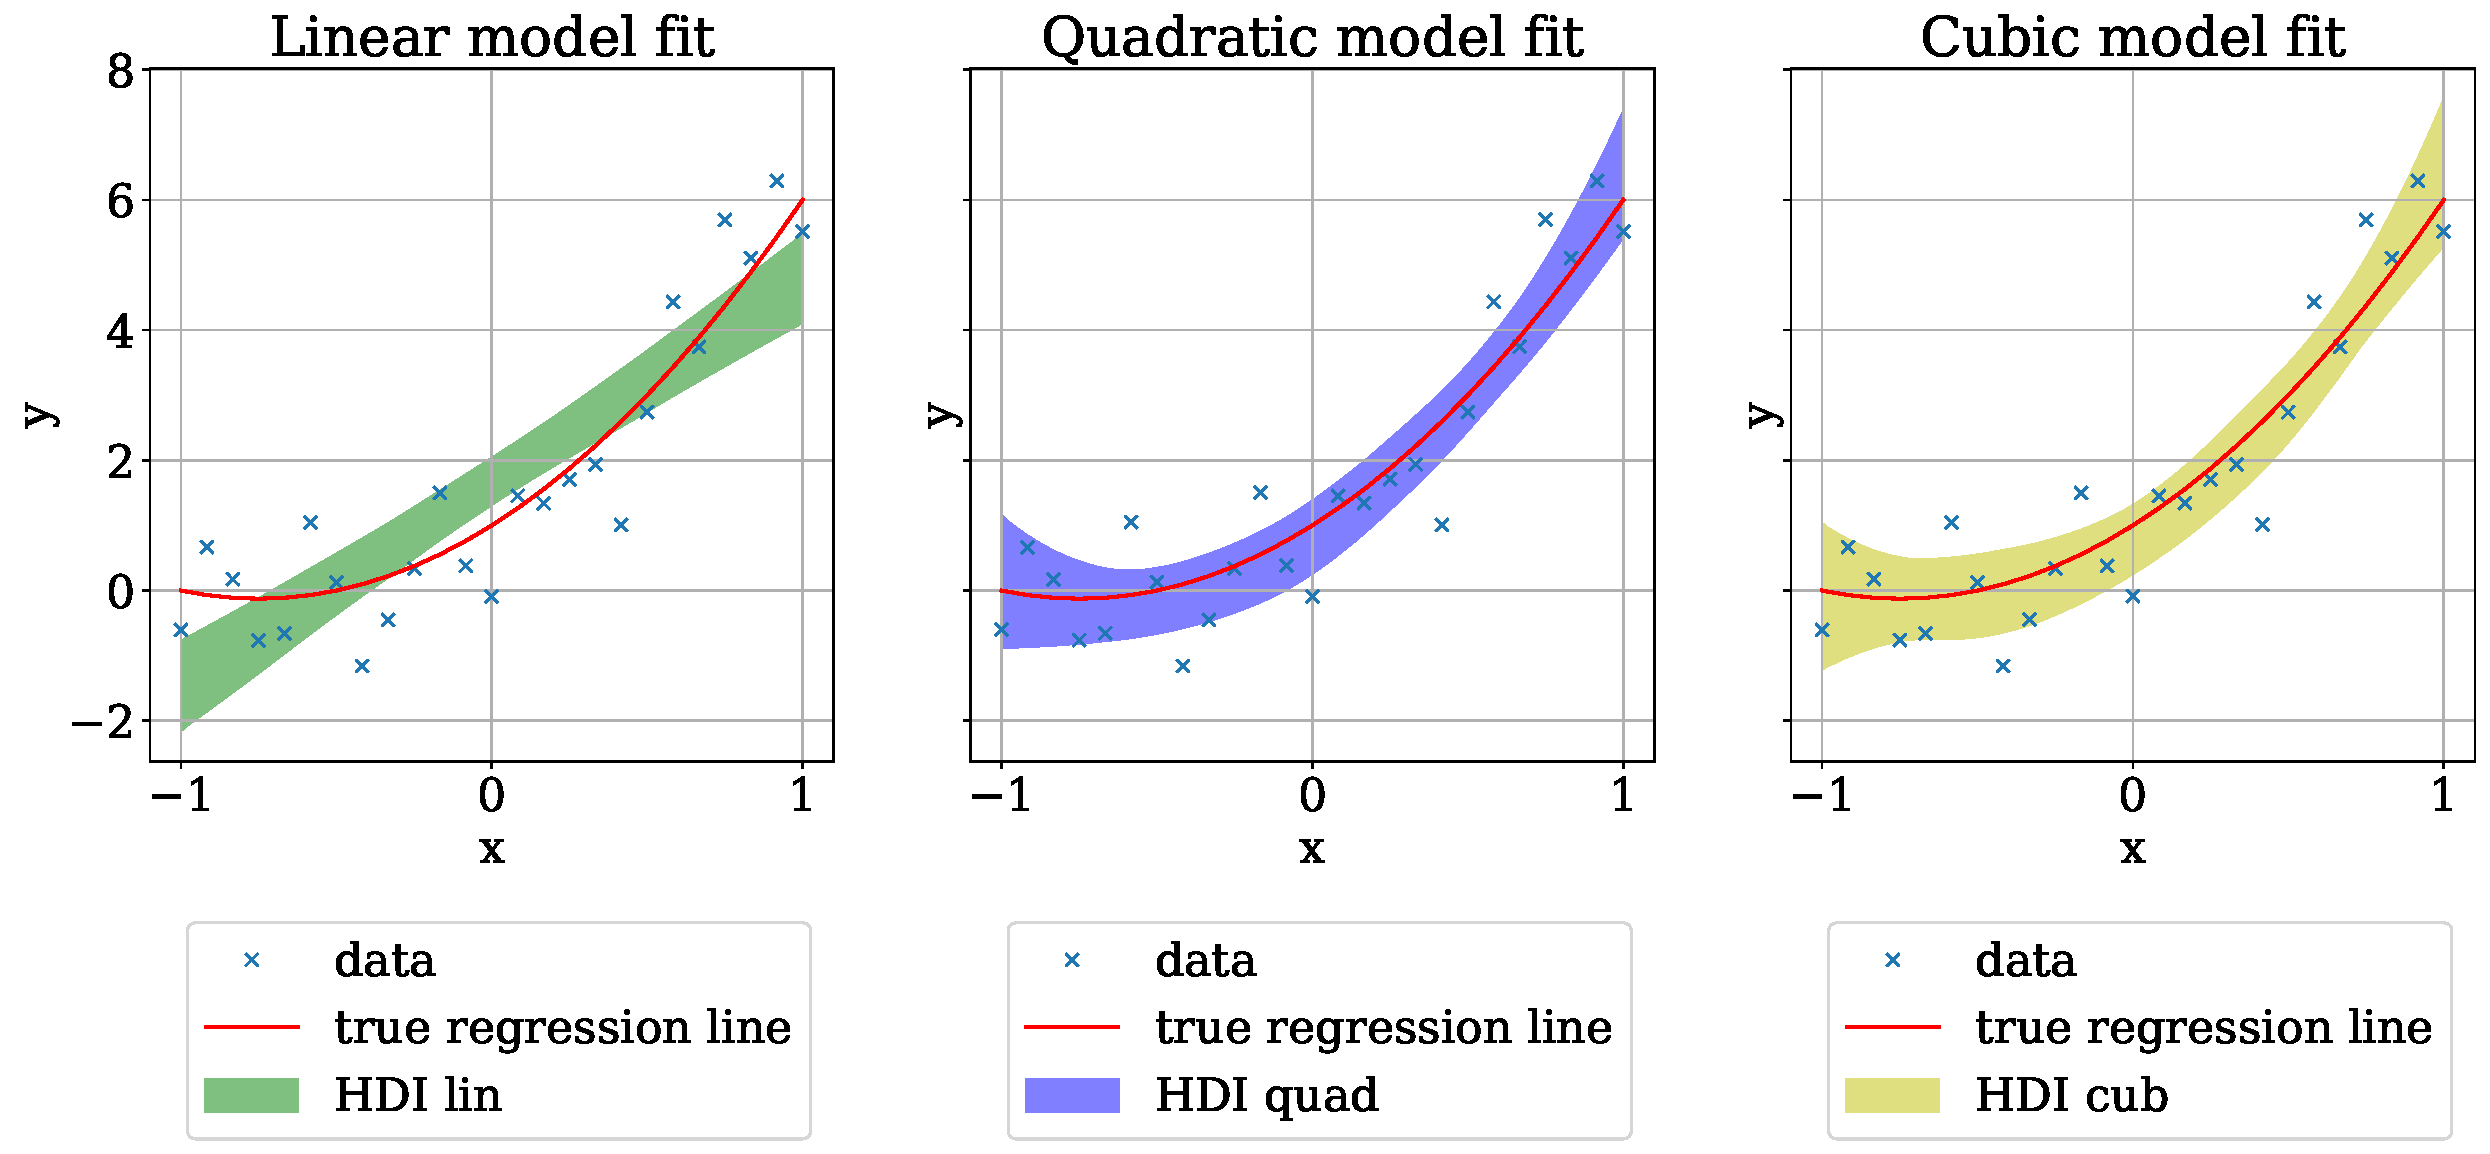
\includegraphics[width=0.8\linewidth]{figs/HDI_sigma_07a.pdf}
	\vfill
	\begin{minipage}{\linewidth}
		\centering
		\begin{minipage}{0.45\linewidth}
			\centering
			\textsc{Dominic Schüchter}\\
			\scriptsize \href{mailto:dschuechter@uni-bonn.de}{\faEnvelope  \hspace*{0.1cm}dschuechter@uni-bonn.de} {\color{black}$|$} \href{https://github.com/dschuechter}{\faGithub  \hspace*{0.1cm}dschuechter}\\
		\end{minipage}
%		$|$
		\begin{minipage}{0.45\linewidth}
			\centering
			\textsc{Jakob Krause}\\
			\scriptsize \href{mailto:krause@hiskp.uni-bonn.de}{\faEnvelope  \hspace*{0.1cm}krause@hiskp.uni-bonn.de} {\color{black}$|$} \href{https://github.com/krausejm}{\faGithub  \hspace*{0.1cm}krausejm}\\
		\end{minipage}
	\vspace{.5cm}
	
	Tutor: \textsc{Andreas Wirzba}\\
	\scriptsize \href{mailto:a.wirzba@fz-juelich.de}{\faEnvelope  \hspace*{0.1cm}a.wirzba@fz-juelich.de}
	\end{minipage}
	\vspace{0.2cm}
	
	19.03.2021
	 
	
%	  \makebox[0pt][l]{\hspace{-7cm}
%	 	\raisebox{0.2cm}[0pt][0pt]{%
%	 		
\includegraphics[width=2.5cm]{pics/UniBonnLogoWithTextMod.png} }}
 		
\end{frame}

%\begin{frame}[plain]
%	\maketitle
%	\setcounter{page}{0}
%\end{frame}

\section*{Introduction}
\begin{frame}{Introduction}
	\begin{tcolorbox}[colback=black!5,colframe=gray!15!black,title=\textsc{Bayes'} Theorem] 
		$$\text{prob}(\btheta|y)=p(\btheta|y)= \frac{p(y|\boldsymbol{\theta})\cdot p(\boldsymbol{\theta})}{p(y)}$$
		with
		\begin{itemize}
			\item \emph{posterior} $p(\btheta|y)$\\
			\item \emph{likelihood} $p(y|\boldsymbol{\theta})$\\
			\item \emph{prior} $p(\boldsymbol{\theta})$\\
			\item \emph{marginal likelihood} $p(y)=\int_{-\infty}^{+\infty}\text{d}\boldsymbol{\theta} p(y|\boldsymbol{\theta})p(\boldsymbol{\theta})$\\
		\end{itemize}
	\begin{center}
		\textbf{This can be used for \emph{model selection} (?)}
	\end{center}
\end{tcolorbox}
\end{frame}


\section*{Table of Contents}

\begin{frame}{Table of Contents}
	\tableofcontents
\end{frame}

\section{Theory}
\subsection{Parameter estimation}
\begin{frame}{Parameter estimation}
	\textsc{Jan} and \textsc{Marius} already talked about this, so here we only sketch the basics again
	\begin{equation}
		\label{eq:marp}
		p(\theta_i|y,M)=\int p(\boldsymbol{\theta}|y,M)\prod_{j\neq i}\text{d}{\theta_j}
	\end{equation}

\begin{align}
	\begin{split}
		p(\theta|y,M)=\max \Leftrightarrow \theta=\hat{\theta}\\
		\langle\theta\rangle=\int_{-\infty}^{\infty}\text{d}\theta  p(\theta|y,M)\cdot\theta
	\end{split}
\end{align}
\end{frame}

\subsection{Model comparison}
\begin{frame}{Model comparison}

	
	\begin{minipage}{.48\linewidth}
		\begin{tcolorbox}[colback=black!5,colframe=gray!15!black,title=\textsc{Bayes} factor] 
			\begin{equation}
			p(M_i|y)=\frac{p(M_i)\cdot p(y|M_i)}{p(y)}.
			\end{equation}
			\begin{align}\label{eq:bf}
			\begin{split}
			O_{ij}&:=\underbrace{\frac{p(M_i|y)}{p(M_j|y)}}_{\text{posterior odds}}\\&=\underbrace{\frac{p(y|M_i)}{p(y|M_j)}}_{\text{\textsc{Bayes} Factor}}\cdot\underbrace{\frac{p(M_i)}{p(M_j)}}_{\text{prior odds}}\\&=B_{ij}\cdot\frac{p(M_i)}{p(M_j)}.
			\end{split}
			\end{align}
		\end{tcolorbox}
	\end{minipage}
\hfil
\begin{minipage}{.45\linewidth}
		How do we turn \textsc{Bayes'} theorem into a tool for model comparison?
	\begin{table}[htbp]
		
		\centering
		{\renewcommand{\arraystretch}{1.3}
			\begin{tabular}{|c|c|c|}
				\hline
				$|\ln B_{ij}|$& Odds  & Strength of evidence \\
				\hline
				$< 1.0$& $ \lesssim 3:1$  & Inconclusive  \\
				$1.0$ & $\sim 3:1$  & Weak evidence  \\
				$2.5$& $\sim 12:1$  & Moderate evidence \\
				$5.0$& $\sim 150:1$ & Strong evidence \\
				\hline
		\end{tabular}}
		\caption{Empirical scale for evaluating the strength of evidence when comparing two models $M_i$ vs. $M_j$, adapted from \citet{Trotta_2008}}
		\label{tab:bf}
	\end{table}
\end{minipage}
	




\end{frame}

\begin{frame}{Model comparison}

	\begin{tcolorbox}[colback=black!5,colframe=gray!15!black,title=\textsc{Bayesian} complexity] 
		\begin{equation}\label{eq:Bayes_Complexity}
			\mathcal{C}_b=-2\int \text{d}\boldsymbol{\theta} p(\boldsymbol{\theta}|y,M)\log(\mathcal{L}(\boldsymbol{\theta}))+2\log(\mathcal{L}(\boldsymbol{\tilde{\theta}})),
		\end{equation}
	
		\begin{equation}\label{eq:Bayes_Complexity_alt}
		\mathcal{C}_b=\overline{\chi^2(\boldsymbol{\theta})}-\chi^2(\boldsymbol{\tilde{\theta}}),
	\end{equation}
	\end{tcolorbox}
\end{frame}

\section{Methods}

\subsection{Monte-Carlo-Sampling}
\begin{frame}{Monte-Carlo-Sampling}
	\begin{minipage}{\linewidth}
		\begin{minipage}{0.6\linewidth}
			\begin{tcolorbox}[colback=black!5,colframe=gray!15!black,title={Benefits of Monte-Carlo-Sampling}] 
				 \begin{equation}
					\langle \boldsymbol{\theta}\rangle\approx \int p(\boldsymbol{\theta} | y)\boldsymbol{\theta}d\boldsymbol{\theta}=\frac{1}{N}\sum_{t=0}^{N-1}\boldsymbol{\theta}^{(t)},
				\end{equation}
				 \begin{equation}
					\langle f(\boldsymbol{\theta})\rangle\approx\frac{1}{N}\sum_{t=0}^{N-1}f(\boldsymbol{\theta}^{(t)}).
				\end{equation}
				also, \emph{marginal posterior} distributions are obtained trivially by binning values of $\theta_i$ ignoring $\theta_{j\neq i}$
			\end{tcolorbox}
		\end{minipage}
		\hfill
		\begin{minipage}{0.3\linewidth}
			\begin{figure}
				
\includegraphics[width=\linewidth]{arviz_logo}
				\vspace{0.1cm}
				
				
\includegraphics[width=\linewidth]{PyMC3_banner}
				\caption{\texttt{ArviZ} \citet{ArviZ} and \texttt{PyMC3} \citet{PyMC3}}
			\end{figure}
			
		\end{minipage}
	\end{minipage}
	
	
\end{frame}
\begin{frame}{Monte-Carlo-Sampling}
	But how exactly do we get samples $\btheta^{(t)}$?
			\begin{tcolorbox}[colback=black!5,colframe=gray!15!black,title={Sequential Monte Carlo (SMC)}]
				First let us introduce an auxiliary \emph{temperature parameter} $\beta\in [0,1]$ and write
				$$p(\btheta|y)_\beta=\frac{p(y|\btheta)^\beta\cdot p(\btheta)}{Z_\beta},$$
				with $Z_\beta=\int\text{d}\btheta p(y|\btheta)^\beta\cdot p(\btheta)$.
				
				Main idea: gradually sample from simple distribution ($\beta=0$) to complex/true distribution ($\beta=1$) using \textsc{Metropolis-Hastings}
				
				SMC then allows us to estimate the \emph{marginal likelihood} as 
				\begin{equation}\label{eq:with_the_hat}
				\hat{p}(y)=\prod_{i}\widehat{\frac{Z_{\beta_i}}{Z_{\beta_{i-1}}}}.
				\end{equation}
		\end{tcolorbox}
\end{frame}


\subsection{\textsc{Savage-Dickey}-Density-Ratio (SDDR)}
\begin{frame}{\textsc{Savage-Dickey}-Density-Ratio (SDDR)}
	consider model $M_j$ with free parameters $\omega,\psi$ and a submodel $M_i$ with one free parameter $\psi$ and fixed $\omega=\omega_\star$. Let us further assume separable priors (which is usually the case \citet{trotta}) $$p(\omega,\psi|M_j)=p(\omega|M_j)p(\psi|M_i).$$
	We can then write the \textsc{Bayes} factor as \citet{trotta} \begin{equation}
	\label{eq:sddr}
	B_{ij}=B_{ji}^{-1}=\frac{p(\omega|y,M_j)}{p(\omega|M_j)}\bigg|_{\omega=\omega_\star}  \text{\hfill (SDDR)}.
	\end{equation}
\end{frame}
%\subsection{Error analysis and diagnostics}
%\begin{frame}{Error analysis and diagnostics}
%To evaluate the errors for the computed quantities we estimate the statistical error given by multiple \emph{Monte-Carlo} runs. Since the results matched our expectations, we are not considering systematic errors in our code. This can be said, because we chose the true models of the underlying data.
%
%To check whether the \textsc{Markov} chains converge, we used the \texttt{ArviZ}-Library that provides functions to visualize \emph{marginal posteriors} and \textsc{Markov} chains \citet{ArviZ}. 
%\end{frame}

\section{Examples}

\subsection{Coin Flip}
\begin{frame}{Coin Flip }
	\begin{itemize}
		\item remember the flipping of a biased coin from the lecture
		\item we want to verify that the coin is biased by using the \textsc{Bayes} factor
		\item two models: $M_1$ -- assumes a fair coin, $M_2$ -- assumes biased coin
	\end{itemize}
	\begin{tcolorbox}[colback=black!5,colframe=gray!15!black,title=Posterior of the coin flip problem]
		\begin{equation}
			p(\theta|y,M_i)=\frac{p(y|\theta,M_i)\cdot p(\theta|M_i)}{\color{red}p(y|M_i)}
		\end{equation}
		to get $p(y|M_i)=\int_{-\infty}^{+\infty}\text{d}{\theta} p(y|{\theta},M_i)p({\theta}|M_i)$ we need to specify a \emph{prior} $p({\theta}|M_i)$ and a \emph{likelihood}  $p(y|{\theta},M_i)$
	\end{tcolorbox}
\end{frame}

\begin{frame}{Coin Flip }
	\begin{minipage}{.49\linewidth}
		\begin{tcolorbox}[colback=black!5,colframe=gray!15!black,title=Choosing a prior]
			\begin{align*}f(\theta;\alpha,\beta)&=\frac{\Gamma(\alpha+\beta)}{\Gamma(\alpha)\Gamma(\beta)}\theta^{\alpha-1}(1-\theta)^{\beta-1}\\&:=\frac{1}{B(\alpha,\beta)}\theta^{\alpha-1}(1-\theta)^{\beta-1}.
			\end{align*}
		\end{tcolorbox}
	\end{minipage}
\hfill
	\begin{minipage}{.49\linewidth}
			\begin{figure}[htbp]
			\centering
			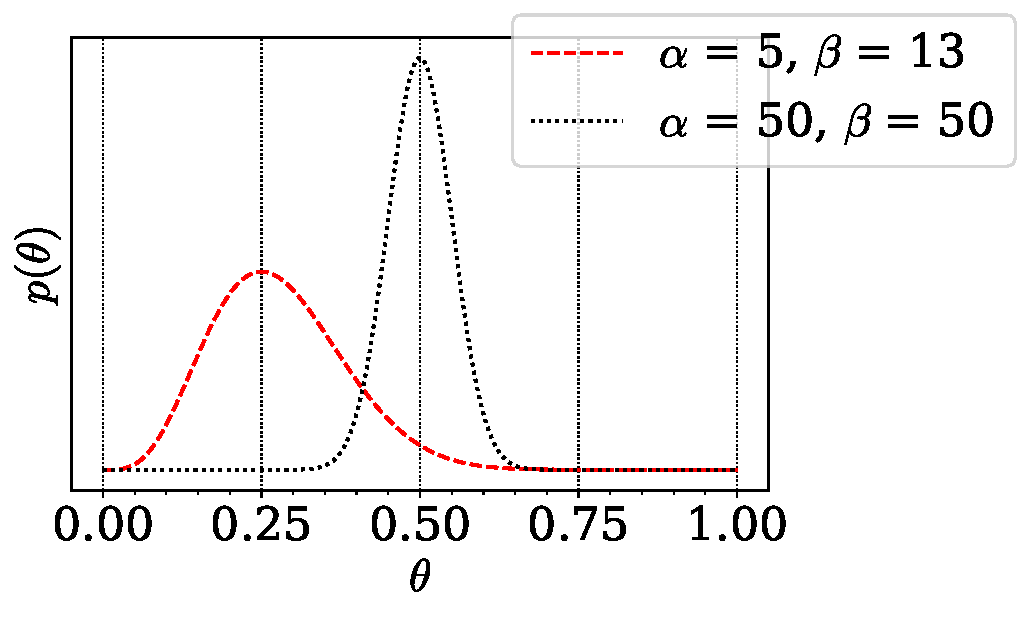
\includegraphics[width=\linewidth]{beta_dist}
			\caption{Beta-distribution as \emph{prior} $p(\theta|M_i)$ for the two different models}
			\label{fig:beta_dist}
		\end{figure}	
	\end{minipage}

\end{frame}

\begin{frame}{Coin Flip}
		\begin{tcolorbox}[colback=black!5,colframe=gray!15!black,title=Choosing a likelihood]
			Since we can assume i.i.d. outcomes of the coin flip a natural choice is a \emph{Binomial distribution}.
			If we observe $k$ heads out of $N$ coin throws ($y=(N,k)$) $$p(y|\theta,M_i)=\begin{pmatrix}N\\k
			\end{pmatrix}\theta^k(1-\theta)^{N-k}.$$
		\end{tcolorbox}
We simulated data for $N=50$ and the biased coin with $p(H)=0.25$.
\end{frame}

\begin{frame}{Coin Flip}
	\begin{tcolorbox}[colback=black!5,colframe=gray!15!black,title=Finally computing the \textsc{Bayes} factor]
		\begin{align*}
		p(y|M_i)&\propto \int_{0}^{1} \text{d}\theta \frac{1}{B(\alpha,\beta)} \cdot \theta^{\alpha+k-1}\cdot (1-\theta)^{N-k+\beta-1}
		=\frac{B(\alpha+k,\beta+N-k)}{B(\alpha, \beta)}\\
		\Rightarrow B_{21}&=B_{12}^{-1}=\frac{B(\alpha_2+k,\beta_2+N-k)\cdot B(\alpha_1,\beta_1)}{B(\alpha_1+k,\beta_1+N-k)\cdot B(\alpha_2,\beta_2)}=9.5839
		\end{align*}
	\end{tcolorbox}
Can we reproduce this numerically?
\end{frame}
\begin{frame}{Coin Flip}
	let us obtain 2000 samples from the posterior distribution using the same \\ \emph{likelihood} and \emph{priors} via the SMC algorithm provided by \texttt{PyMC3}
	\begin{figure}[htbp]
		\begin{subfigure}{.49\linewidth}
			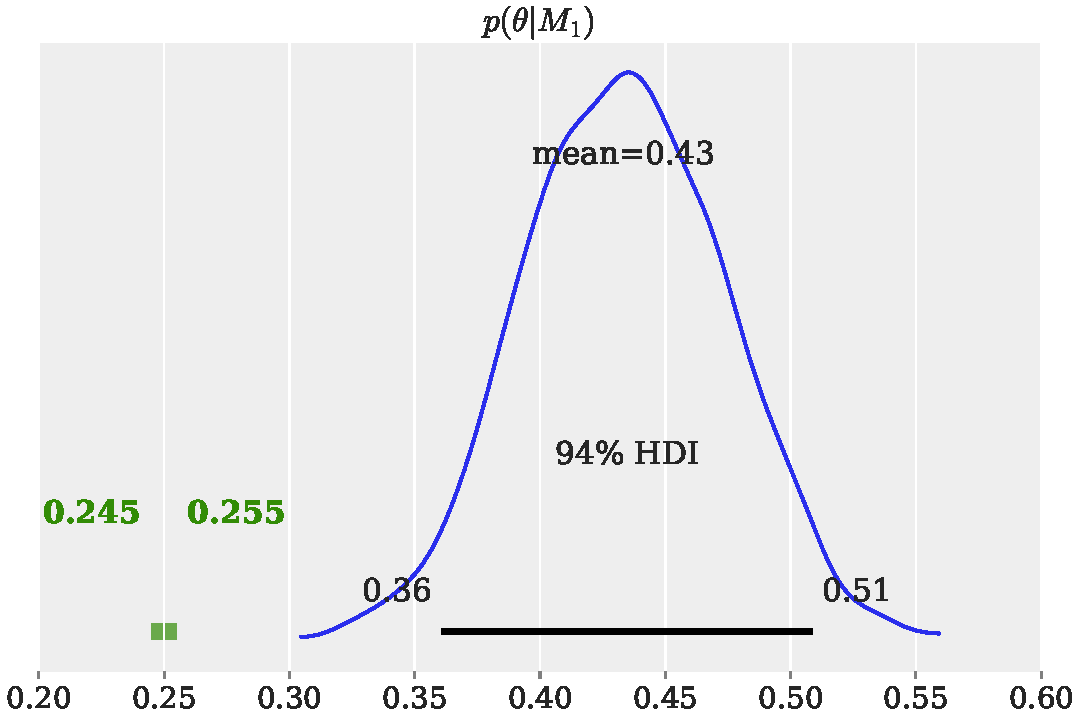
\includegraphics[width=0.9\linewidth]{coin_marp_m1.pdf}
			\subcaption{}\label{fig:coin_marp_a}
		\end{subfigure}
		\begin{subfigure}{.49\linewidth}
			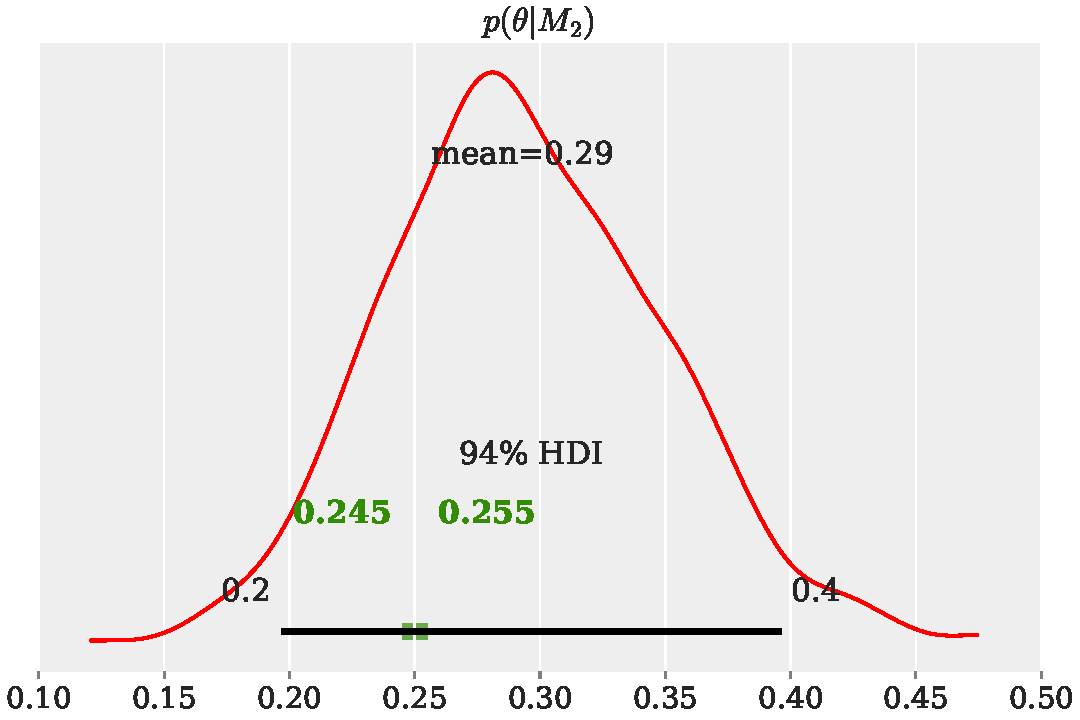
\includegraphics[width=0.9\linewidth]{coin_marp_m2.pdf}
			\subcaption{}\label{fig:coin_marp_b}
		\end{subfigure}
		\caption{The \emph{marginal posterior} for $\alpha=\beta=50$ \eqref{fig:coin_marp_a} and $\alpha=5, \beta=13$ \eqref{fig:coin_marp_b} of 2000 samples. HDI means highest density interval. The highlighted green intervals denote the expected value.}\label{fig:coin_marp}
	\end{figure}
 $$\text{We find }B_{21}=B_{12}^{-1}=9.5829\pm0.4719  \text{ (noice! } \checkmark)$$
\end{frame}
\subsection{Fitting a polynomial of unknown degree}
\begin{frame}{Fitting a polynomial of unknown degree}
	We wish to determine the true model underlying the generated data depicted in the figure below

		\centering
		\begin{minipage}{.7\linewidth}
			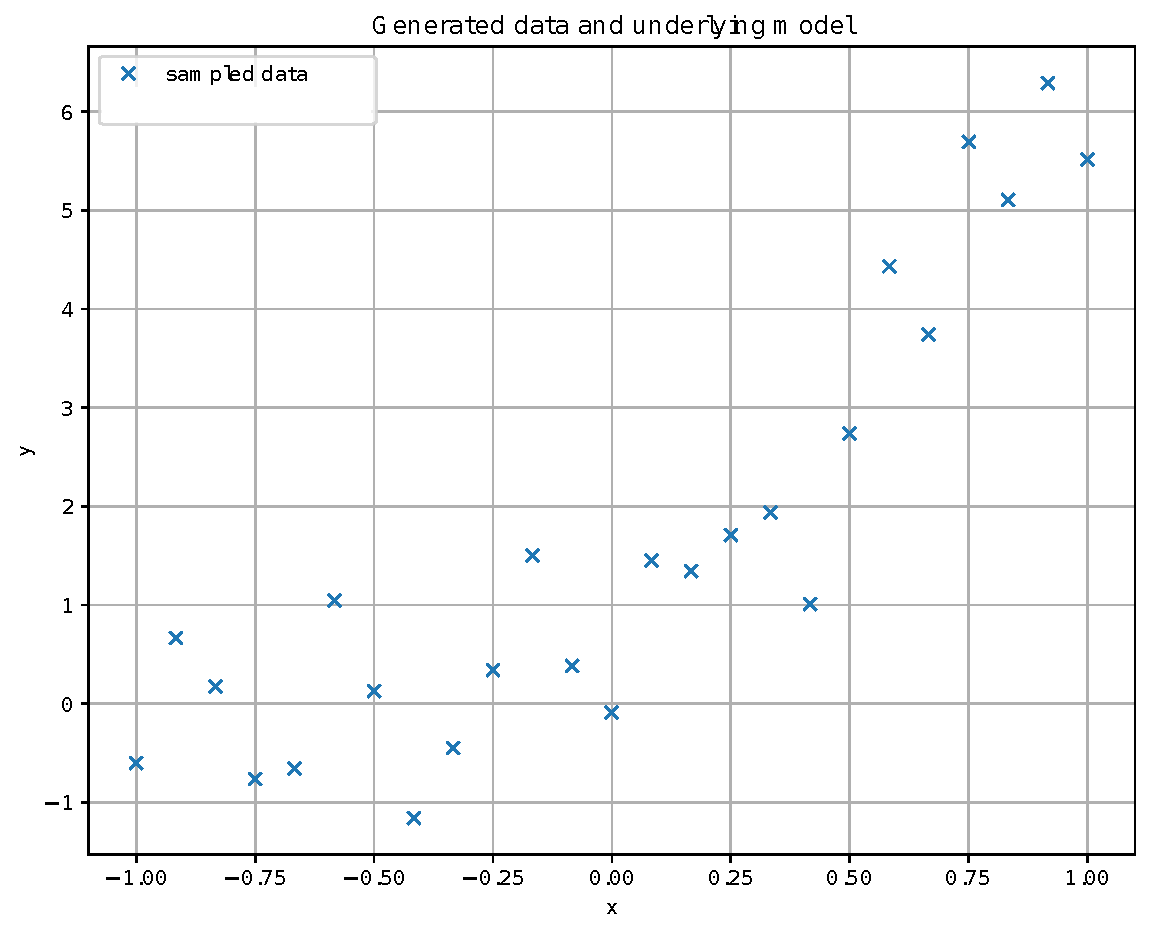
\includegraphics[width=.9\linewidth]{data_regression_line_sigma_07a_data.pdf}
		\end{minipage}
		\begin{minipage}{.25\linewidth}
				\begin{figure}
						\caption{$N=25$ datapoints distributed with a gaussian noise of $\sigma=0.7$. Linear? Quadratic? Cubic?}
				\end{figure}
		\end{minipage}

	
	
\end{frame}

\begin{frame}{Fitting a polynomial of unknown degree}
	we want to find the correct model by using
	
	\begin{itemize}
		\item \textsc{Bayes} factor 
		\item SDDR (as sanity check)
		\item \textsc{bayesian} complexity
	\end{itemize}
	We will tackle this problem numerically by sampling from the \emph{posterior} $\to$ we need to assign \emph{priors} and \emph{likelihoods} again
\end{frame}

\begin{frame}{Fitting a polynomial of unknown degree}
	a suitable choice for \emph{prior} and \emph{likelihood} are normal distributions, since the noise is Gaussian \citet{sivia}.
		\begin{tcolorbox}[colback=black!5,colframe=gray!15!black,title=Choosing a prior]
		The \emph{priors} for the fit-parameters $a,b$ and $c$  are each described by a normal distribution with $\mu_{\text{prior}}=0$ and $\sigma_{\text{prior}}=2$
	\end{tcolorbox}

		\begin{tcolorbox}[colback=black!5,colframe=gray!15!black,title=Choosing a likelihood]
			$$p(y|\btheta, M_i)=\prod_{k=1}^{N}\frac{1}{\sigma\sqrt{2\pi}}\exp{\left[-\frac{(f(y_k;\btheta)-y_k)^2}{2\sigma^2}\right]}.$$
			where $f(y_k;\btheta)$ is the fit function $f_i(x)=\displaystyle\sum_{\alpha=0}^{i}a_\alpha x^\alpha$, with $i=1,2,3$
	\end{tcolorbox}
\end{frame}

\begin{frame}{Fitting a polynomial of unknown degree}
	Now lets generate 2000 samples following the \emph{posterior}
	\begin{figure}
		\centering
		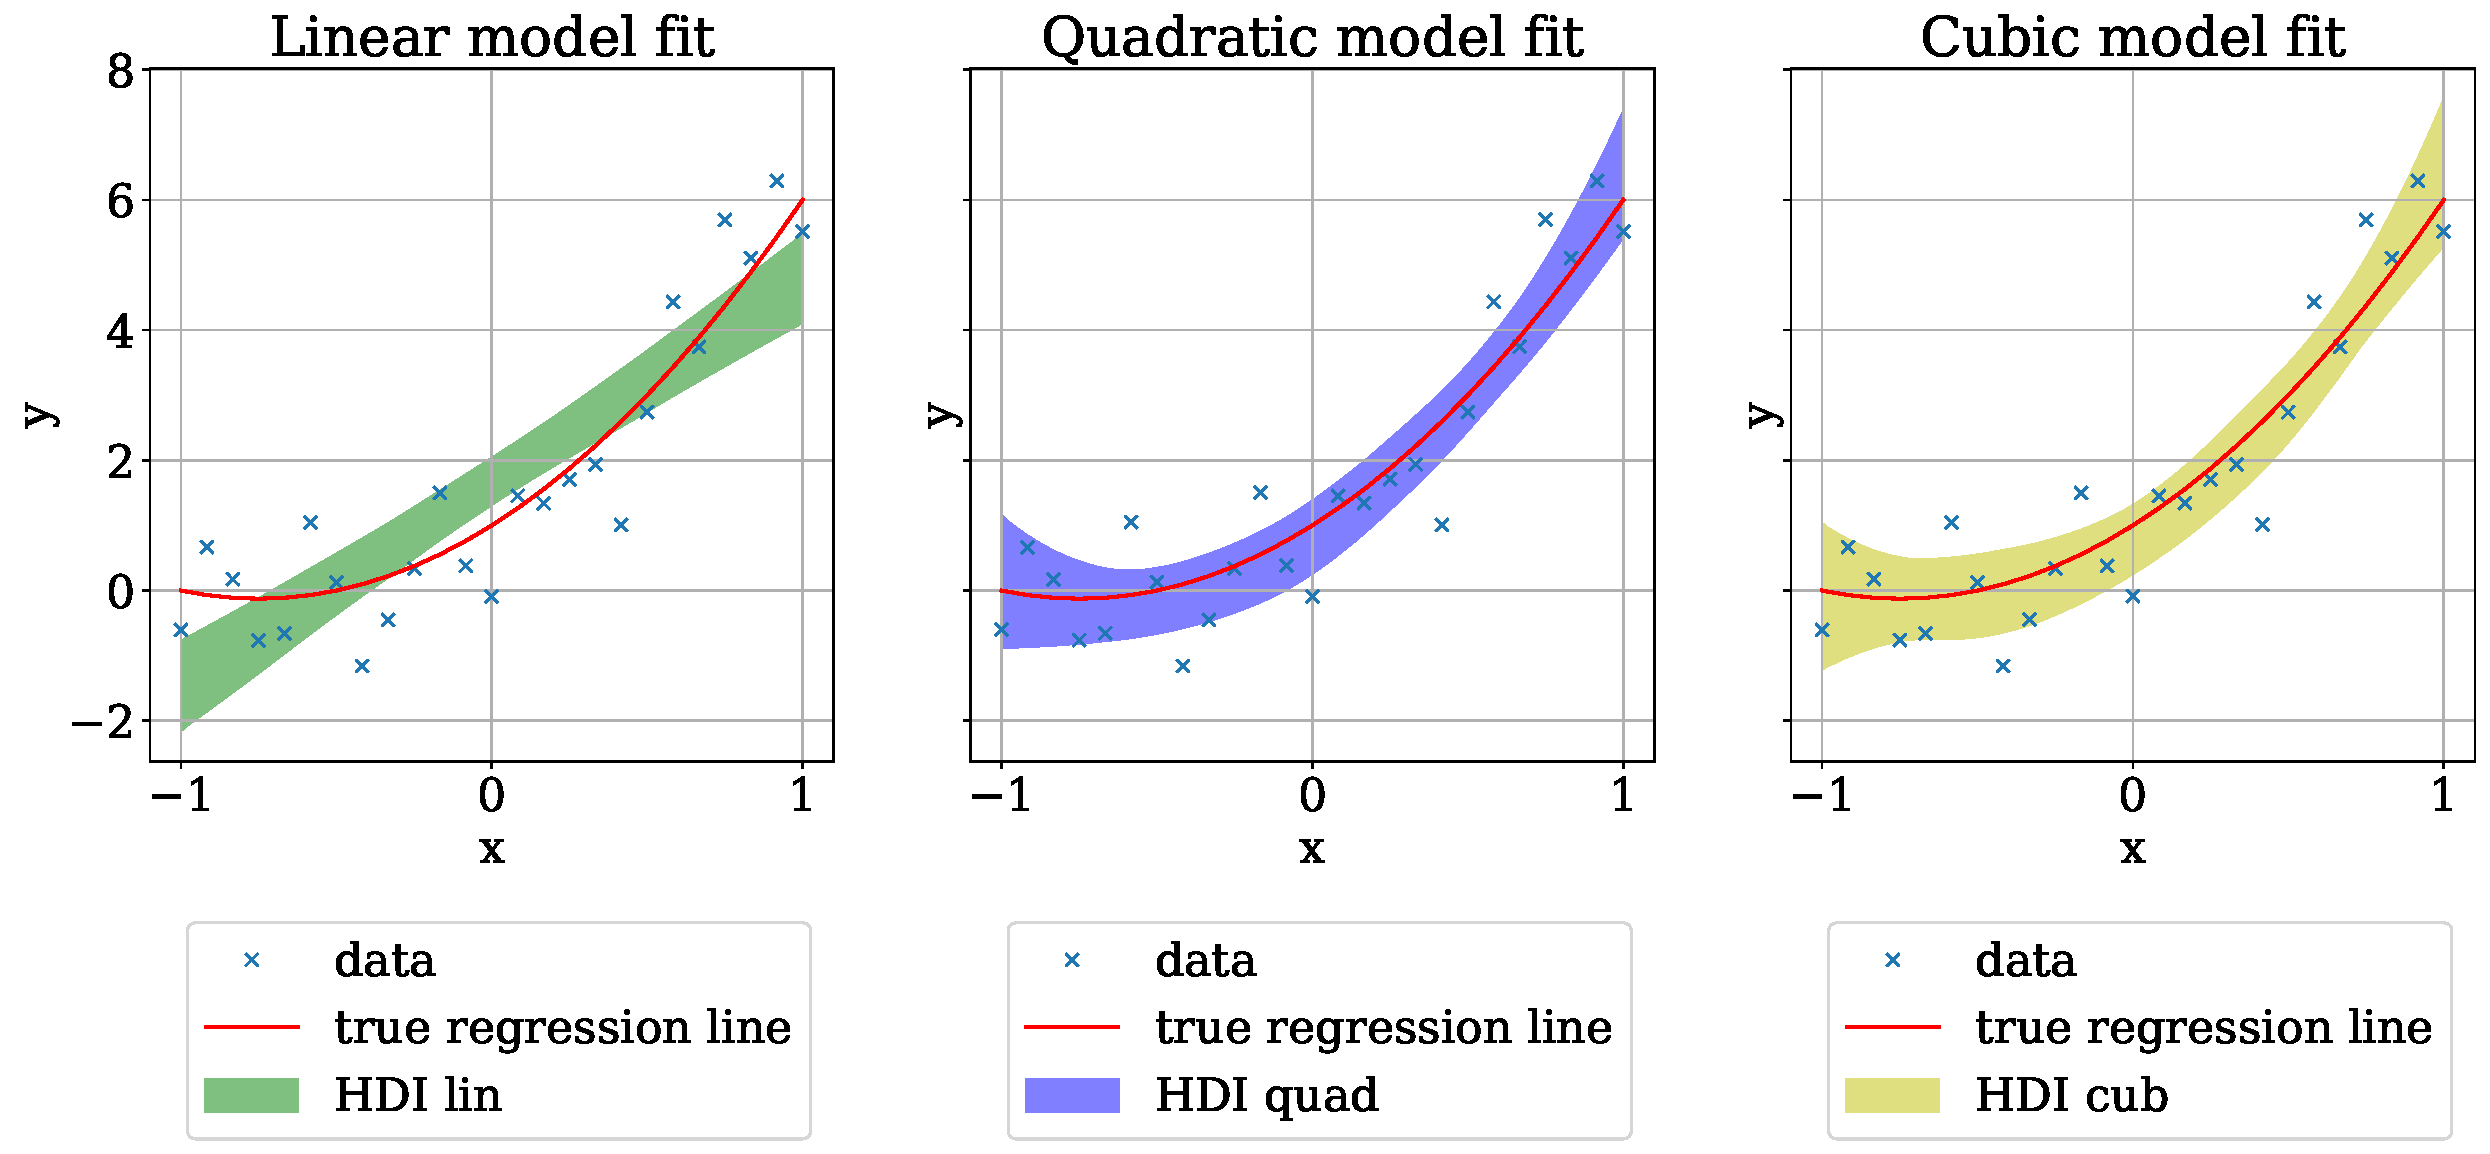
\includegraphics[width=\linewidth]{figs/HDI_sigma_07a.pdf}
		\caption{Result of parameter estimation with SMC. The data was generated with $\sigma=0.7$}
	\end{figure}
\end{frame}
\begin{frame}{Fitting a polynomial of unknown degree}
	\begin{minipage}{.49\linewidth}

		\begin{table}[H]
			{\renewcommand{\arraystretch}{1.3}
				\resizebox{\columnwidth}{!}{
				\begin{tabular}{|c|c|}
					\hline
					Comparison $M_1$ vs. $M_2$ & $\ln(B_{12}(\sigma=0.7))$  \\
					\hline
					square vs. linear& $8.5507\pm0.053$\\
					cubic vs. linear & $7.6225\pm0.094$\\
					square vs. cubic&$0.9371\pm0.1093$ \\
					\hline
			\end{tabular}}}
			\caption{Results of \textsc{Bayes} factor via SMC}
			\label{tab:res_smc}
		\end{table}
	
		\begin{table}[H]
			{\renewcommand{\arraystretch}{1.3}
				\resizebox{\columnwidth}{!}{
				\begin{tabular}{|c|c|}
					\hline
					Comparison $M_1$ vs. $M_2$ & $\ln(B_{12}(\sigma=0.7))$ \\
					\hline
					square vs. linear& $>2.4301\pm0.27613$\\
					square vs. cubic&$0.8091\pm0.0265$  \\
					cubic vs. linear & $>0.3329\pm0.1292$\\
					\hline
			\end{tabular}}}
			\caption{Results of \textsc{Bayes} factor via SDDR.}
			\label{tab:res_sddr}
		\end{table}
	
	\end{minipage}
	\begin{minipage}{.49\linewidth}
		\begin{figure}[H]
			\centering
			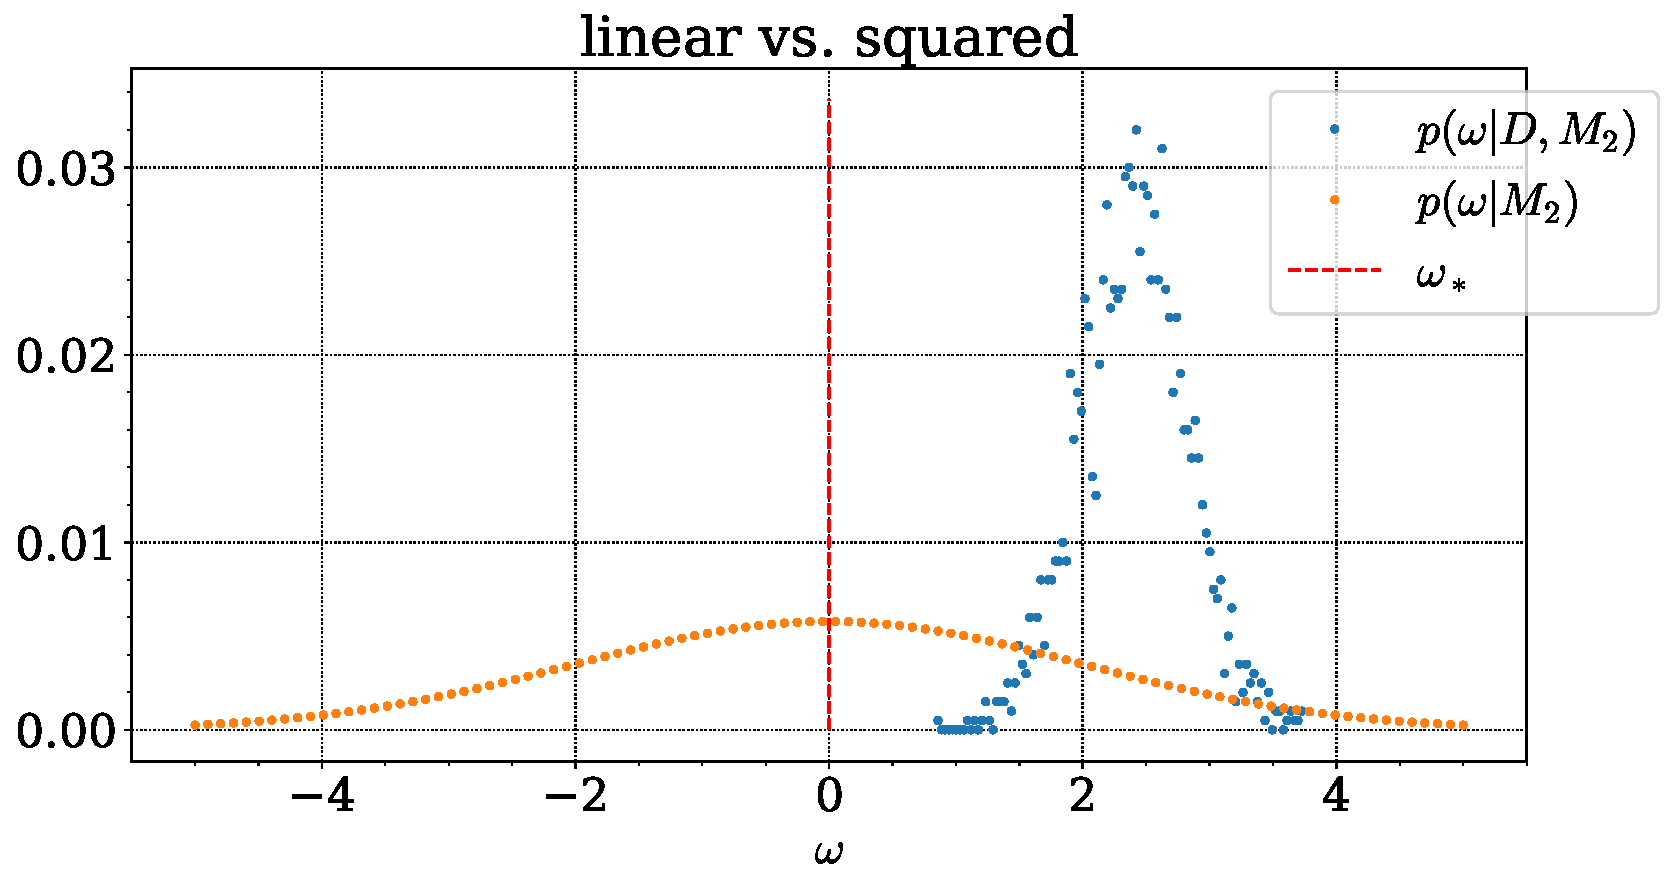
\includegraphics[width=\linewidth]{SDDR_linear vs. squared_sigma_07a+.pdf}
			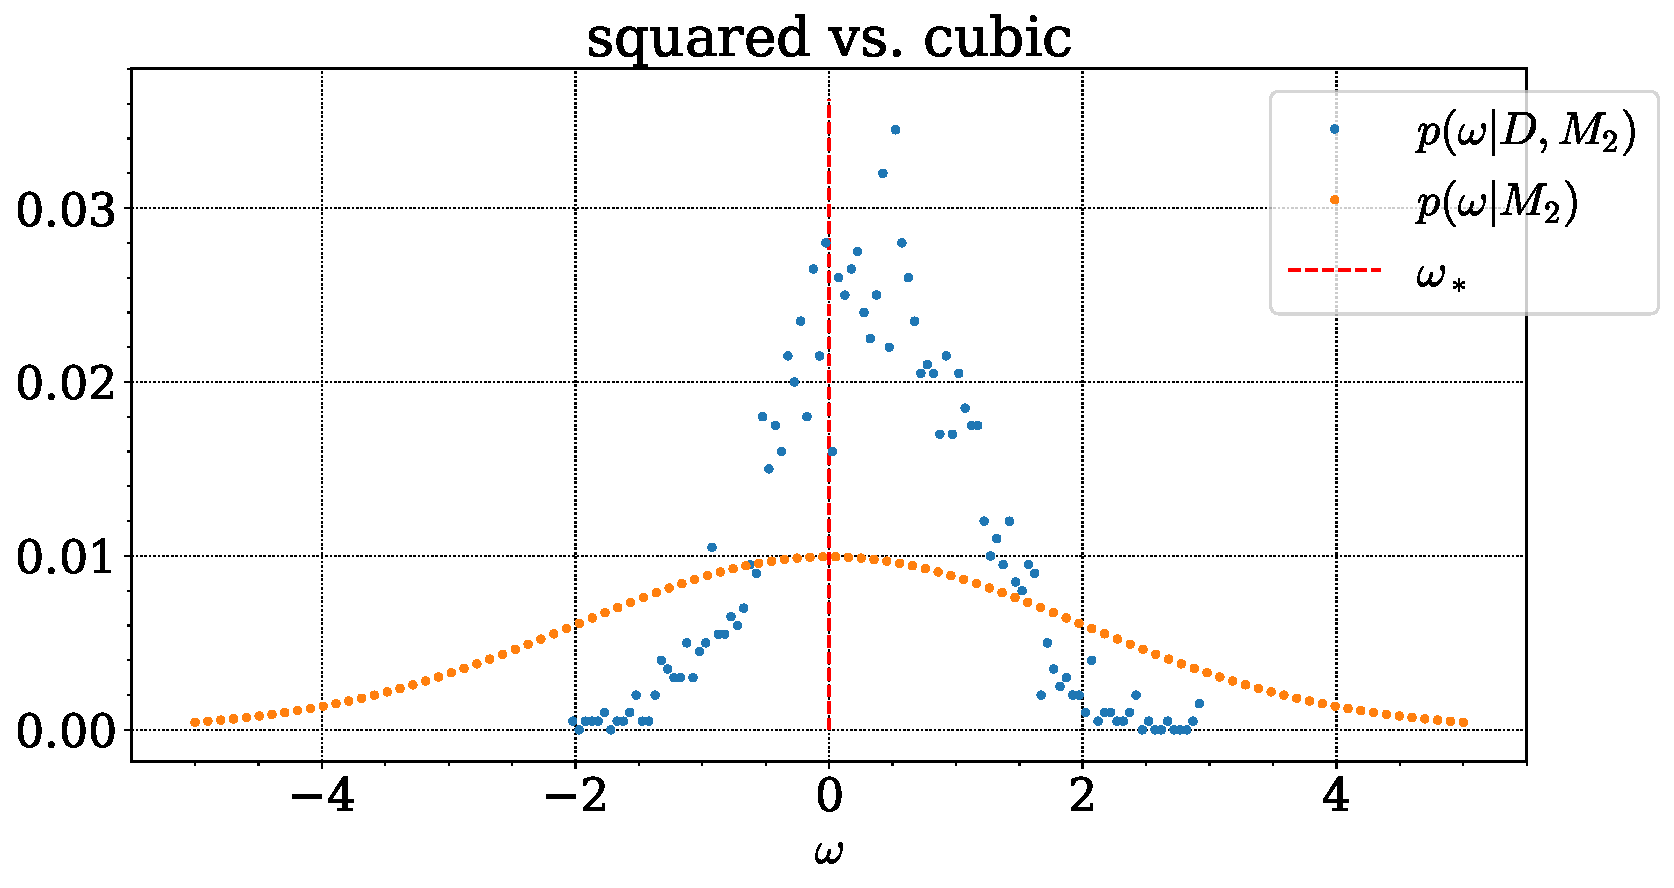
\includegraphics[width=\linewidth]{SDDR_squared vs. cubic_sigma_07a+.pdf}
			\caption{Computation of the SDDR  ($\sigma=0.7$)}
			\label{fig:sddr}
		\end{figure}
	\end{minipage}

\end{frame}
\begin{frame}{Fitting a polynomial of unknown degree}
	What about the complexity?
	\begin{figure}
		\centering
		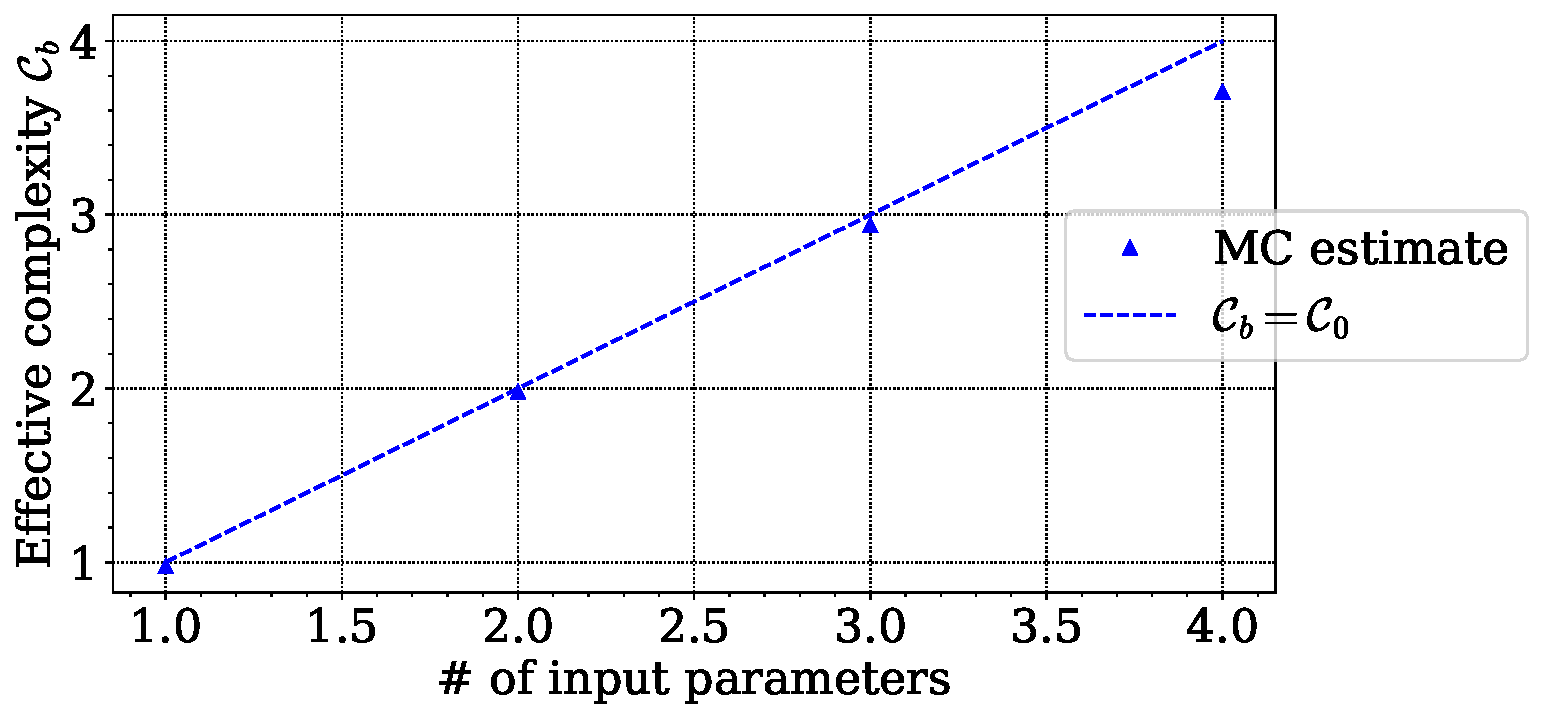
\includegraphics[width=\linewidth]{_sigma_07acomplexity.pdf}
		\caption{Numerical computation of the complexity $\mathcal{C}_b$, 3 parameters are supported.}
	\end{figure}
\end{frame}

\begin{frame}{Fitting a polynomial of unknown degree}
	And the true regression line is...
	
	\begin{minipage}{.6\linewidth}
	\begin{figure}
		\centering
		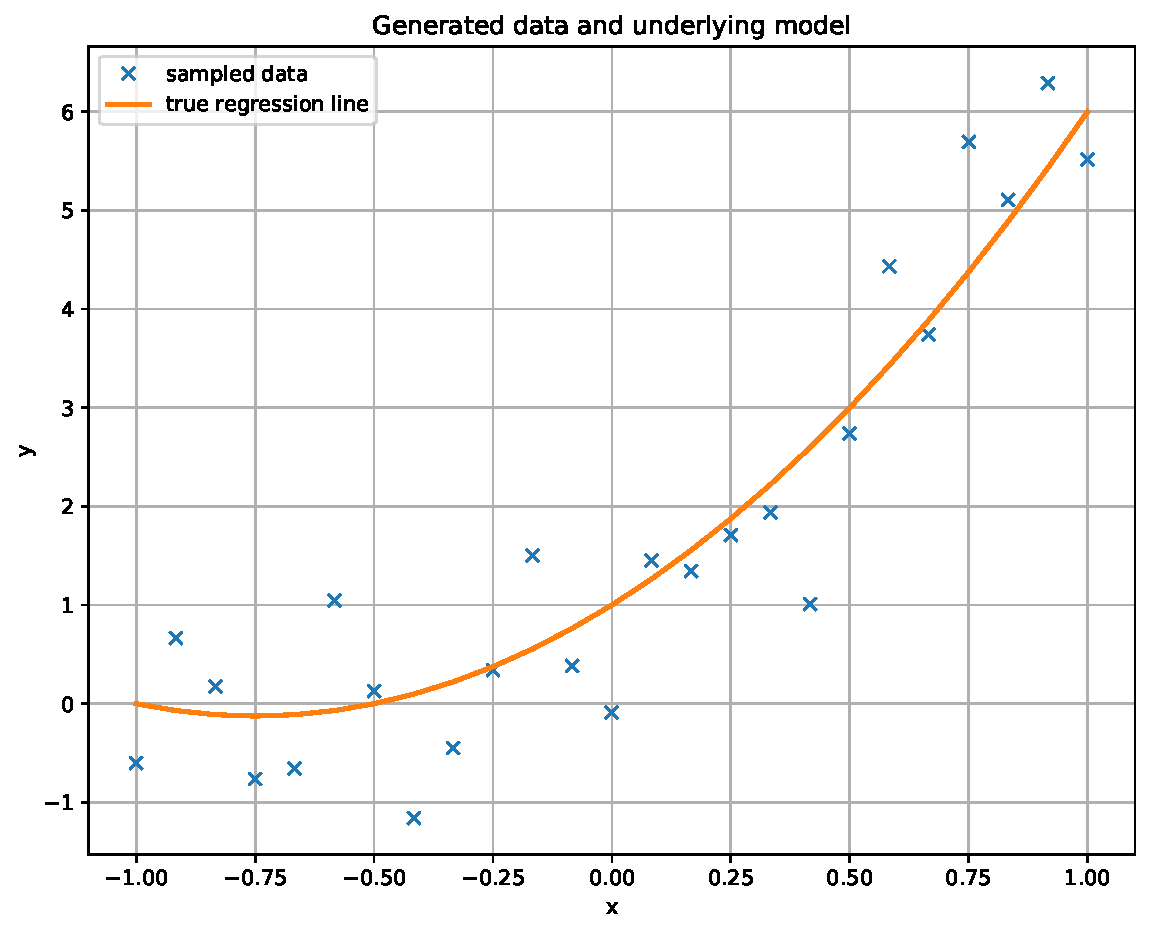
\includegraphics[width=\linewidth]{data_regression_line_sigma_07a}
		\caption{True regression line}
	\end{figure}
	\end{minipage}
\begin{minipage}{.39\linewidth}
	\begin{align*}
	f(x;\btheta)&=a\cdot x^2+b\cdot x+c\\&=2\cdot x^2+3\cdot x+1.
	\end{align*}
	\centering
	\text{ (again, nice!} $\checkmark$)
\end{minipage}
	

\end{frame}

\section{Summary}
\begin{frame}{Summary}
	\begin{tcolorbox}[colback=black!5,colframe=gray!15!black,title=, width=\linewidth]
		\begin{itemize}
			\item 
		\end{itemize}
	\end{tcolorbox}
\end{frame}

\section*{References}
\begin{frame}[allowframebreaks]{References}
	\setbeamertemplate{bibliography item}[text]

	\printbibliography
\end{frame}

\end{document}